% !TEX encoding = UTF-8 Unicode

\linespread{1.7}
\chapter{Calibration of the Near-surface Seismic Structure in the SCEC Community Velocity Model Version 4}
\linespread{2.0}
%\newrefsection
\label{chap:highf}

\graphicspath{{/Users/zhh076/work/PhD_way/high_f/}}

The near-surface seismic structure (to a depth of about 1000 m), particularly the shear-wave velocity (Vs), can strongly affect the propagation of seismic waves, and therefore must be accurately calibrated for ground motion simulations and seismic hazard assessment. The Vs of the top ~30 m of the crust (Vs30) is often well-characterized from borehole studies, geotechnical measurements, and water wells, while the velocities of the material deeper than about 1000 m are typically determined by tomography studies. However, the material parameters between these two regions are typically poorly constrained due to lack of data constraints. A widely-used method for incorporating the near-surface earth structure is incorporated in the Southern California Earthquake Center (SCEC) Community Velocity Models (CVMs) by interpolating Vs from Vs30 measurements to the S-wave velocity at 350 m \citep{elyVs30derivedNearsurfaceSeismic2010}. However, our 3D simulations of the 2014 M5.1 La Habra earthquake in the Los Angeles area using the SCEC CVM-S4.26.M01 model significantly underpredict low-frequency (< 1 Hz) ground motions at rock sites for the \citet{elyVs30derivedNearsurfaceSeismic2010} method. On the other hand, extending the Vs30-based refinement of the shallow velocities down to a depth of about 1000 meters improves the fit between our synthetics and seismic data at rock sites considerably, without compromising the fit at soil sites. We recommend that our proposed near-surface velocity refinement at rock sites down to about 1000 meters be incorporated in CVM-S4.26M01, as well as considered for other CVMs.


%%%%%%%%%%%%%%%%%%%%%%%%%%
\section{Introduction} \label{introduction}



%%%%%%%%%%%%%%%%%%%%%%%%%%%%%%%
\section{Numerical Approach}\label{approach}


%%%%%%%%%%%%%%%%%%%%%%%%%%%%%%


\section*{Data and Resources}
The UCVM program used to extract velocity meshes can be obtained from SCEC on \url{https://github.com/SCECcode/UCVMC} (last accessed 12/2020). The simulations were performed on Summit at the Oak Ridge Leadership Computing Facility in Tennessee. Most of the data-processing work was done using Python and the Generic Mapping Tools package (\url{https://www.generic-mapping-tools.org}, last accessed 04/2021).


\section*{Acknowledgements}
\addcontentsline{toc}{section}{\protect\numberline{}Acknowledgements}

This research was supported through the U.S. Geological Survey External Program (award \#G19AS00021), as well as the Southern California Earthquake Center (SCEC; Contribution Number xx). SCEC is funded by the National Science Foundation (NSF) Cooperative Agreement EAR-1600087 and the U.S. Geological Survey (USGS) Cooperative Agreement G17AC00047. We thank Robert W. Graves for providing the source models and Fabio Silva for providing the station records of the 2014 La Habra earthquake.

\Cref{chap:highf}, in full, is a reformatted version of a paper currently being prepared: Hu, Z. and Olsen, K.B. (2021), 0-5 Hz Deterministic 3D Ground Motion Simulations for the 2014 Mw 5.1 LaHabra Earthquake. The dissertation author was the primary investigator and author of this paper.

\newpage
\section*{Tables and Figures}
\addcontentsline{toc}{section}{\protect\numberline{}Tables and Figures}%

%% For very long table
% \clearpage
% \begin{sidewaystable}[!ht]
% \caption{Coregionalization matrix $\mathbf{P}^\mathbf{3}$}
% \begin{adjustbox}{width=\textwidth,center}
% \begin{tabular}{|c|cccccccccccccccccccccccccccccccc|c|}
% \end{tabular}
% \label{tb:5-S3}
% \end{adjustbox}
% \end{sidewaystable}



% %%%%%%%%%%%%% figures 

\clearpage
\floatsetup[figure]{style=plain,subcapbesideposition=top,font=Large}
% \captionsetup[figure]{justification=justified,
%     labelfont={color={magenta},bf},textfont={color={green}},
%     labelsep=newline}
\begin{figure}[!ht]
    \sidesubfloat[]{\includegraphics[width=0.9\textwidth]{topo_q100f06_ely1000_hist.pdf}\label{fig:highf-7a}} \\[1.2\baselineskip]% %\hfil
    \sidesubfloat[]{\includegraphics[width=0.9\textwidth]{topo_q100f06_hist.pdf}\label{fig:highf-7b}} %% \\[\baselineskip]% $$\hfil
    \caption{ (a) $V_S$ profile sample locations in California. Triangles denote rock sites and circles denote soil sites, and (b) extracted $V_S$ profiles. The top panel zooms into the top 500 m. }
    \label{fig:highf-7}
\end{figure}

% \clearpage
% \floatsetup[figure]{style=plain,subcapbesideposition=top,font=Large,footfont=Large}
% \begin{figure}[!ht]
%     \sidesubfloat[]{\includegraphics[width=0.4\textwidth]{figures/figure_vs30_14a.png}\label{fig:vs30-14a}} \hfil
%     \sidesubfloat[]{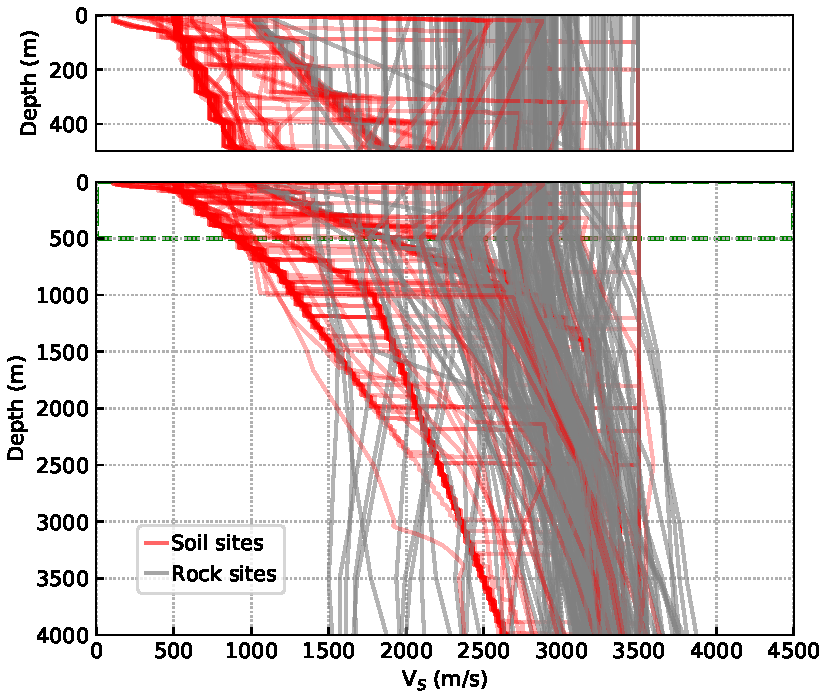
\includegraphics[width=0.45\textwidth]{figures/figure_vs30_14b.pdf}\label{fig:vs30-14b}} % \\[\baselineskip]%
%     \caption{ (a) $V_S$ profile sample locations in California. Triangles denote rock sites and circles denote soil sites, and (b) extracted $V_S$ profiles. The top panel zooms into the top 500 m. }
%     \label{fig:vs30-14}
% \end{figure}
% \clearpage

%% supplement
\setcounter{table}{0}
\setcounter{figure}{0}
\numberwithin{figure}{chapter}
\numberwithin{table}{chapter}
\renewcommand{\thetable}{S\arabic{chapter}.\arabic{table}}
\renewcommand{\thefigure}{S\arabic{chapter}.\arabic{figure}}
\newpage
\section*{Supplementary Materials}
\addcontentsline{toc}{section}{\protect\numberline{}Supplementary Materials}

This supplement includes.




\renewcommand{\thetable}{\arabic{table}}
\renewcommand{\thefigure}{\arabic{figure}}

\numberwithin{figure}{chapter}
\numberwithin{table}{chapter}

%\endrefsection